\subsection{Aperçu de l'expressivité de \nameTool\label{sec:sat_tobedone}}

\paragraph{Ensembles de domaines}
Avec le temps, nous avons remarqué que nous avions souvent besoin d'écrire des choses comme :
$$\begin{aligned}\bigwedge_{i \in \{1..9\}} \bigwedge_{j \in \{1..9\}}\bigwedge_{ m\in \{A,B,C,D,E,F,G,H,I\}} \hspace{2cm}\\ \left( P_{i,j,m}\IMPL \bigwedge_{n \in \{A,B,C,D,E,F,G,H,I\}|m\neq n}\NOT P_{i,j,n}\right)\end{aligned}$$
Si on lit $P_{i,j,m}$ comme  ``il y a la lettre $m$ dans la case $(i,j)$'' d'une grille $9\times 9$, la formule ci-dessus exprime qu'il y a \emph{au plus} une lettre parmi `A' ... `I' dans chaque case. 

Ces ensembles $\{1..9\}$ et $\{A,B,C,D,E,F,G,H,I\}$ sont des \emph{ensembles de domaines}, et avec \nameTool\ l'utilisateur peut définir autant d'ensembles de domaines qu'il le souhaite, par exemple :

\begin{verbatim}
  $N=[1..9]
  $L=[A,B,C,D,E,F,G,H,I]
\end{verbatim}

et ainsi écrire la formule précédente comme :
$$\bigwedge_{i \in N} \bigwedge_{j \in N}\bigwedge_{ m\in L}P_{i,j,m}\IMPL \bigwedge_{n \in L|m\neq n}\NOT P_{i,j,n}$$
De plus, les opérations usuelles sur les ensembles ($\cup$, $\cap$, $\setminus$, \ldots) peuvent être utilisées pour définir d'autres ensembles.


\paragraph{Formules propositionnelles}

Les formules de \nameTool\ sont basées sur des variables propositionnelles (qui peuvent être indicées) et les opérateurs logiques usuels ($\AND$, $\OR$, $\IMPL$, $\NOT$, $\IFF$). Ainsi on peut taper des formules usuelles simples comme $Pluie \IMPL Nuages$. Mais en plus, nous fournissons des opérateurs logiques de haut niveau qui permettent d'exprimer des assertions complexes dans une forme très compacte.

\paragraph{Conjonctions et disjonctions généralisées}
Elles permettent d'exprimer des conjonctions et des disjonctions sur des formules contenant des paramètres qui varient, par exemple :
\begin{itemize}
\item $ \bigwedge_{i \in N} P_i$, o\`u $N$ est l'ensemble de domaine défini précédemment.\\
  Elle représente la conjonction
  $P_1 \AND P_2 \AND \ldots \AND P_9$. 
\item $\bigvee_{i \in E} P_i$.
\end{itemize}

Bien s\^ur, ces opérateurs peuvent être imbriqués comme dans :
$$\bigwedge_{i \in N} \bigwedge_{j \in N}\bigvee_{ m\in L}P_{i,j,m}$$

qui indique que dans chaque cellule se trouve au moins une lettre.


\paragraph{Contraintes de cardinalité}
Il s'agissait de l'un des sujets "laissé pour le futur" de \cite{GaScSt2011}.
Ces opérateurs logiques moins classiques sont disponibles dans \nameTool\ : il permettent de réduire drastiquement la taille de certaines formules, ce sont : $\atM{}{}$, $\atL{}{}$ et $\exact{}{}$.\\ L'exemple suivant décrit leur signification :
\begin{itemize}
\item $\atM{i \in N}{2} P_i$ représente ``pour au plus deux valeurs de $i \in N$ $P(i)$ est vraie'';
\item $\atL{i \in N}{2} P_i$ représente ``pour au moins deux valeurs de $i \in N$ $P(i)$ est vraie'';
\item $\exact{i \in N}{2} P_i$ représente ``pour exactement deux valeurs de $i \in N$ $P(i)$ est vraie''.
\end{itemize}
La disjonction généralisée est en fait un cas particulier de ceci (au moins une est vraie), la conjonction aussi (au plus 0 est fausse), et le ou exclusif peut être vu comme exactement une parmi deux est vraie. \\
Rappelons qu'avec des opérateurs logiques classiques et avec $N$ contenant 9 éléments, $\atM{i \in N}{3} P_i$ devrait nécessiter une formule contenant 84 propositions $P_i$ puisque cela revient à choisir 3 parmi 9 ce qui donne $\binom{9}{3}$ possibilités, et ni $\bigwedge$ ni $\bigvee$ n'aideraient beaucoup. 

\paragraph{Contraintes et calculs sur des indices}

Souvent, nous avons besoin d'ajouter des contraintes sur les indices, par exemple :
$$\bigwedge_{i \in E } \bigwedge_{j \in E  | i \neq j}P_{i,j}$$
qui signifie que $P_{i,j}$ est vraie lorsque $i\neq j$. 

Il s'agissait de la seule contrainte disponible dans \satoulouse, maintenant dans \nameTool\ la gamme de possibilités à été largement enrichie. Les contraintes peuvent inclure des opérateurs usuels de comparaison comme $<$, $>$, $\leq$, $\geq$, $\neq$, $=$ et ces comparaisons peuvent s'appliquer non seulement aux indices, mais aussi à toute expression arithmétique impliquant des indices et $+$, $-$, $*$, $/$, $\mod$, $\sqrt{\phantom{x}}$. 

Exprimer une phrase comme ``chaque case $(i,j)$ contient un nombre qui n'est pas égal à $i+j$'' donnera :
$$\bigwedge_{i \in N } \bigwedge_{j \in N} \bigvee_{k \in N|k\neq i+j} P_{i,j,k}$$
Bien s\^ur, \emph{toutes ces phrases} pourraient être exprimées avec les opérateurs logiques usuels bruts, mais ceci serait un travail fastidieux. Néanmoins, les étudiants doivent savoir ce qui est derrière la scène, et qu'une telle formule est l'abréviation de quelque chose comme :
$$P_{1,1,1}\vee P_{1,1,3}\vee P_{1,1,4}\ldots P_{1,2,1}\vee P_{1,2,2}\vee P_{1,2,4}\vee \ldots $$
qui est très long et terne.



\subsection{Détails du langage}

\subsubsection{Langage d'entrée vs. langage d'affichage}

Les formules que nous avons vues précédemment sont écrites dans le \emph{langage d'affichage} (style \LaTeX), mais tous ces symboles ne sont pas disponibles sur les claviers, ainsi pour écrire les formules et ensembles de domaines, l'utilisateur utilisera le \emph{langage d'entrée}.
Par exemple, la formule précédente avec l'ensemble associé $N$ sera tapée (les variables sont pr\'{e}fix\'{e}es par \$) :
\begin{verbatim}
bigand $i,$j in $N,$N:
  bigor $k in $N when $k != $i+$j:
    P($i,$j,$k)
  end
end
\end{verbatim}
Mais \nameTool\ les affiche immédiatement en style \LaTeX\ comme on peut le voir dans le panneau droit montr\'{e} sur la figure \ref{fig:LatexDisplay}.
La d\'{e}finition de l'ensemble $N$ est faite dans l'onglet ``Ensembles''.

\begin{figure*}[htbp]
\centering
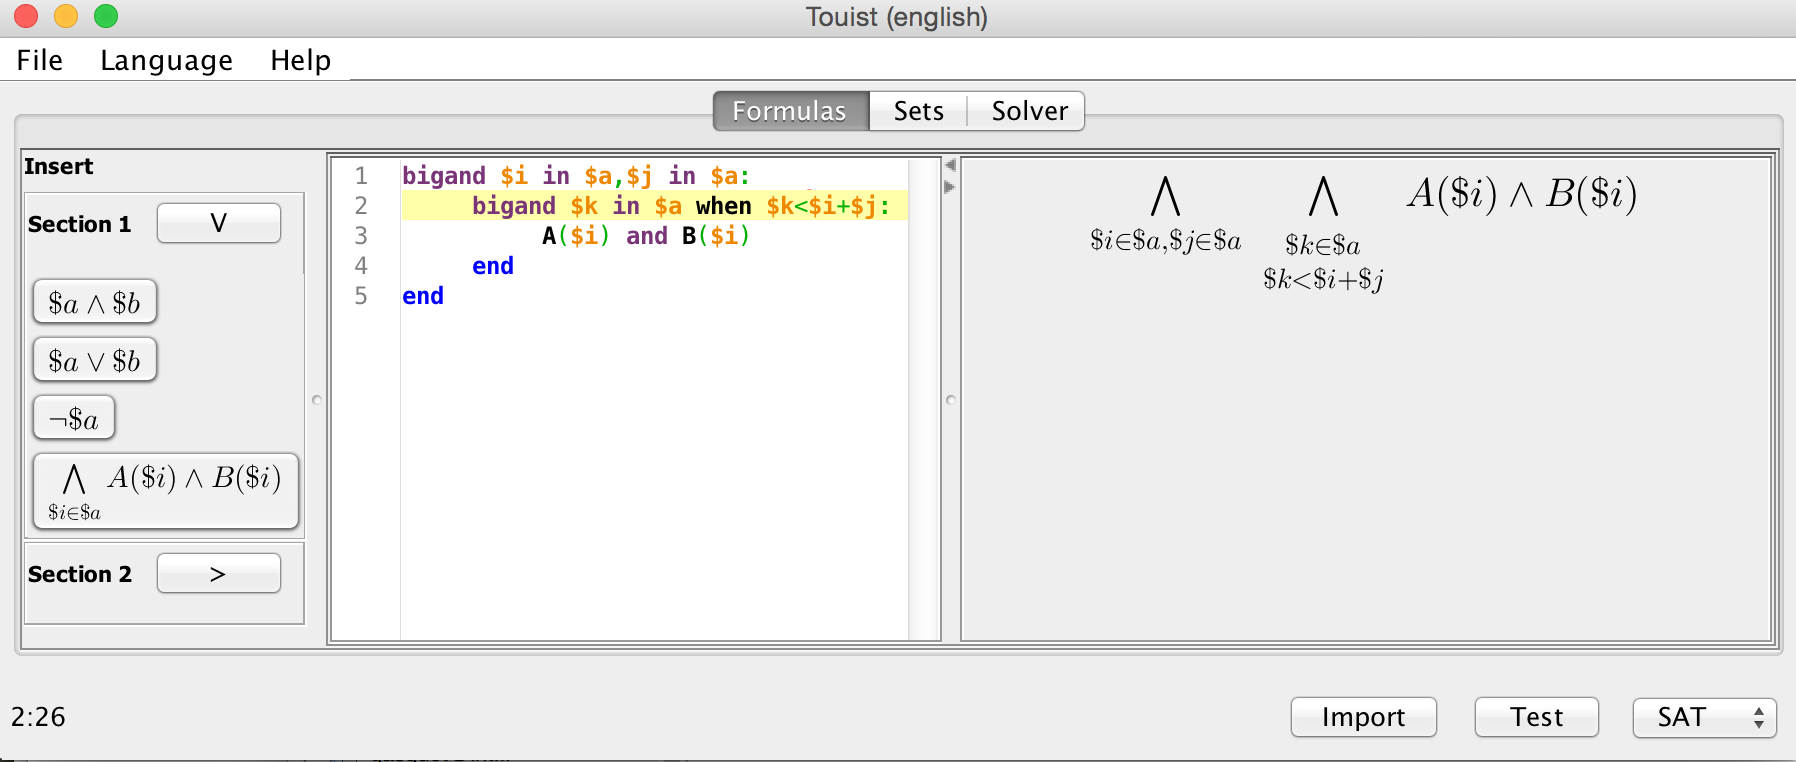
\includegraphics[scale=0.45]{Pictures/LatexDisplay.png}
  \caption{Affichage en style \LaTeX}
  \label{fig:LatexDisplay}
\end{figure*}


En outre, les formules peuvent être tapées à la main dans la fenêtre d'édition, ou introduites dans une sorte d'éditeur dirigé par la syntaxe, en raffinant progressivement l'arbre syntaxique, ou encore elles peuvent être importées à partir d'un fichier externe.





%\begin{figure*}[ht]
%  \centering
%  \includegraphics[scale=.4]{touist1.png}
%  \caption{Interface de TouIST}
%  \label{fig:touist}
%\end{figure*}



%\chapter{Language reference}\label{sec-language-reference}%mdk%mdk

Cette section présente les fonctionnalités liées au langage développé pendant la thèse.

\subsection{Structure d'un fichier {\scshape TouIST} file}\label{sec-structure-of-a-touist-file}%mdk%mdk
\begin{mdpre}%mdk
\noindent{\mdcolor{purple}\textless{}touist-file\textgreater{}}~::=~{\mdcolor{purple}\textless{}assign\textgreater{}}~{\mdcolor{purple}\textless{}touist-file\textgreater{}}\\
~~~~~~~~~~~~~~~~\textbar{}~{\mdcolor{purple}\textless{}formula\textgreater{}}~{\mdcolor{purple}\textless{}touist-file\textgreater{}}\\
~~~~~~~~~~~~~~~~\textbar{}~EOF%mdk
\end{mdpre}\noindent Un fichier {\scshape TouIST} est 
{\color{red} whitespace-separated\footnote{\noindent A whitespace is a space, tab or newline.%mdk
\label{fn-whitespace}%mdk%mdk
} list of
assignments and formulas. Assignments are global and can be interleaved
with formulas as long as they are not nested in formulas (for local
variables, you can use \mdcode{{\mdcolor{navy}let}}; see Sec.~\ref{let-binding}). Comments begin
with "\mdcode{{\mdcolor{darkgreen};;}}". Two backslashes (\mdcode{\textbackslash{}\textbackslash{}}) in a formula will produce a new
line in the latex view.

\noindent\textbf{Note}.
The whitespace-separated list of formulas is actually going to be
converted to a conjunction; it avoids many intermediate \mdcode{and}.
\textbf{Warning:} each formula in this list is going to be put in
parentheses:%mdk
\begin{mdpre}%mdk
\noindent a~or~b\\
c~=\textgreater{}~a%mdk
\end{mdpre}\noindent will be translated to
\begin{mdpre}%mdk
\noindent(a~or~b)~and~(c~=\textgreater{}~a)%mdk
\end{mdpre}\label{newline-and-note}%mdk%mdk

\subsection{Variables}\label{sec-variables}%mdk%mdk

\noindent First, we describe what a variable is. Then, we detail how to assign
variables (with global or local assignments).%mdk

\subsubsection{Syntax of a variable}\label{sec-syntax-of-a-variable}%mdk%mdk
\begin{mdpre}%mdk
\noindent{\mdcolor{purple}\textless{}expr\textgreater{}}~::=~{\mdcolor{purple}\textless{}int\textgreater{}}\textbar{}{\mdcolor{purple}\textless{}float\textgreater{}}\textbar{}{\mdcolor{purple}\textless{}prop\textgreater{}}\textbar{}{\mdcolor{purple}\textless{}bool\textgreater{}}\textbar{}{\mdcolor{purple}\textless{}set\textgreater{}}\\
~~~~\textbar{}~"""{\mdcolor{purple}\textless{}formula-simple\textgreater{}}"""~{\mdcolor{darkgreen}\textless{}-~quoted~formula,~since~TouIST~\textgreater{}=~3.5.1}\\
{\mdcolor{purple}\textless{}var\textgreater{}}~::=~"\$"~TERM~~~~~~~~~~~~~~~~~~~~~~~~~~~~{\mdcolor{darkgreen}\textless{}-~simple-var}\\
~~~~\textbar{}~"\$"~TERM~"("~{\mdcolor{purple}\textless{}comma-list(\textless{}expr\textgreater{})\textgreater{}}~")"~~~{\mdcolor{darkgreen}\textless{}-~tuple-var}%mdk
\end{mdpre}
\begin{mddefinitions}%mdk

\mddefterm{\noindent{\bfseries Simple variable (\textquotedblleft{}simple-var\textquotedblright{})}}%mdk

\begin{mdbmarginx}{}{}{}{1.5em}%mdk
\begin{mddefdata}%mdk
A simple variable is of the form \mdcode{{\mdcolor{purple}\$my\_var}}. In a formula, a simple
variable is always expected to be a proposition or a
\mdref{quoted-formulas}{quoted formula}. In an expression, a simple
variable can contain an integer, a floating-point, a proposition, a boolean
or a set.
%mdk
\end{mddefdata}%mdk
\end{mdbmarginx}%mdk

\mddefterm{\noindent{\bfseries Tuple variable (can be seen as a \emph{predicate})}}%mdk

\begin{mdbmarginx}{}{}{}{1.5em}%mdk
\begin{mddefdata}%mdk
A tuple variable is a simple variable followed by a comma-separated list of
indexes in braces, e.g., \mdcode{{\mdcolor{purple}\$var}({\mdcolor{purple}\$i},a,{\mdcolor{purple}4})}. The leading variable (\mdcode{{\mdcolor{purple}\$var}})
must always contain a proposition. The nested indexes (e.g., \mdcode{{\mdcolor{purple}\$i}})
can be integers, floats, propositions or booleans.
%mdk
\end{mddefdata}%mdk
\end{mdbmarginx}%mdk

\begin{mdbmarginx}{}{}{}{1.5em}%mdk
\begin{mddefdata}%mdk
A tuple variable will always be expanded to a proposition or a
\mdref{quoted-formulas}{quoted formula}. For example, if
\mdcode{{\mdcolor{purple}\$var}=p} and \mdcode{{\mdcolor{purple}\$i}=q}, then it will expand to \mdcode{p(q,a,{\mdcolor{purple}4})}
%mdk
\end{mddefdata}%mdk
\end{mdbmarginx}%mdk

\begin{mdbmarginx}{}{}{}{1.5em}%mdk
\begin{mddefdata}%mdk
Tuple variables are not (yet) compatible with the set-builder construct (in
\ref{set-builder}). If one of the indexes is a set, the set will stay
as-is.%mdk
\end{mddefdata}%mdk
\end{mdbmarginx}%mdk
%mdk
\end{mddefinitions}%mdk

\noindent Here are some examples of variables:%mdk

\begin{mdcenter}%mdk
\begin{mdtabular}{2}{\dimeval{(\linewidth)/2}}{1ex}%mdk
\begin{tabular}{cc}\midrule
{\bfseries Simple-var}&{\bfseries Tuple-var}\\

\midrule
\mdcode{{\mdcolor{purple}\$N}}&\mdcode{{\mdcolor{purple}\$place}({\mdcolor{purple}\$number})}\\
\mdcode{{\mdcolor{purple}\$time}}&\mdcode{{\mdcolor{purple}\$action}({\mdcolor{purple}\$i},{\mdcolor{purple}\$j})}\\
\mdcode{{\mdcolor{purple}\$SIZE}}&\\
\mdcode{{\mdcolor{purple}\$is\_over}}&\\
\midrule
\end{tabular}\end{mdtabular}
%mdk
\end{mdcenter}%mdk

\subsubsection{Global assignment}\label{global-var}%mdk%mdk

\noindent We call \textquotedblleft{}global variables\textquotedblright{} any variable that is assigned at the same
depth as the subformulas of the {\scshape TouIST} formula. A {\scshape TouIST} formula is
the formula formed by the conjunction of each blank-separated {\scshape TouIST}
statement (a blank is a newline, a space or a tabulation). For example,
in the following {\scshape TouIST} formula:%mdk
\begin{mdpre}%mdk
\noindent a~and~(b~or~c)~d~e~=\textgreater{}~f~~~~\\
g~h~\textless{}=\textgreater{}~i\\
k~or~l\\
m%mdk
\end{mdpre}\noindent the subformulas \mdcode{a~and~(b~or~c)}, \mdcode{d}, \mdcode{e~or~f}, \mdcode{h~\textless{}=\textgreater{}~i},
\mdcode{k~or~l} are subformulas of the {\scshape TouIST} formula but \mdcode{(b~or~c)} is not
(instead, it is a sub-subformula).

It is equivalent to%mdk
\noindent\noindent\[  (a \wedge (b \vee c)) \wedge (d) \wedge (e \rightarrow f) \wedge (g)
    \wedge (h \leftrightarrow i) \wedge (k \vee l) \wedge (m)
\]%mdk
\noindent This means that global variables cannot be nested in sub-subformulas;
they must appear at the same \textquotedblleft{}depth\textquotedblright{} as the subformulas. We cannot write
\mdcode{(a~or~({\mdcolor{purple}\$x}=b~{\mdcolor{purple}\$x}))} for example.

The assignment syntax is the following:%mdk
\begin{mdpre}%mdk
\noindent{\mdcolor{purple}\textless{}assign\textgreater{}}~::=~{\mdcolor{purple}\textless{}var\textgreater{}}~"="~({\mdcolor{purple}\textless{}expr\textgreater{}})~~~~~~{\mdcolor{darkgreen}\textless{}--~global~assignment}\\
{\mdcolor{purple}\textless{}expr\textgreater{}}~::=~{\mdcolor{purple}\textless{}int\textgreater{}}\textbar{}{\mdcolor{purple}\textless{}float\textgreater{}}\textbar{}{\mdcolor{purple}\textless{}prop\textgreater{}}\textbar{}{\mdcolor{purple}\textless{}bool\textgreater{}}\textbar{}{\mdcolor{purple}\textless{}set\textgreater{}}\\
~~~~\textbar{}~"""{\mdcolor{purple}\textless{}formula-simple\textgreater{}}"""~~~~~~~~~{\mdcolor{darkgreen}\textless{}--~TouIST~\textgreater{}=~3.5.1}%mdk
\end{mdpre}\noindent Global variables apply for the whole code, even if the assignment is
occurs after the use of the variable. This is because all global
assignments are evaluated before any formula.

The only case where the order of assignment is important is when you
want to use a variable in a global assignment expression. Global
assignments are sequentially evaluated, so the order of assignment
matters. For example:%mdk
\begin{mdpre}%mdk
\noindent{\mdcolor{purple}\$N}~=~{\mdcolor{purple}10}\\
{\mdcolor{purple}\$set}~=~{}[{\mdcolor{purple}1}..{\mdcolor{purple}\$N}]~~~~{\mdcolor{darkgreen};;~\$N~must~be~defined~before~\$set}%mdk
\end{mdpre}
\subsubsection{Local assignment (\mdcode{{\mdcolor{navy}let}} construct)}\label{let-binding}%mdk%mdk

\noindent Sometimes, you want to use the same result in multiple places and you
cannot use a global variable (presented in~\ref{global-var}) because of
nested formulas. The \mdcode{{\mdcolor{navy}let}} construct lets you create temporary
variables inside formulas:%mdk
\begin{mdpre}%mdk
\noindent{\mdcolor{purple}\textless{}let-assign\textless{}T\textgreater{}\textgreater{}}~::=\\
~~~~\textbar{}~"let"~{\mdcolor{purple}\textless{}var\textgreater{}}~"="~{\mdcolor{purple}\textless{}expr\textgreater{}}~":"~{\mdcolor{purple}\textless{}formula\textless{}T\textgreater{}\textgreater{}}~~~~~{\mdcolor{darkgreen}\textless{}--~local~assignment}\\
~~~~\textbar{}~"let"~{\mdcolor{purple}\textless{}comma-list(\textless{}var\textgreater{})\textgreater{}}~"="~{\mdcolor{purple}\textless{}comma-list(\textless{}expr\textgreater{})\textgreater{}}~":"~{\mdcolor{purple}\textless{}formula\textless{}T\textgreater{}\textgreater{}}\\
{\mdcolor{purple}\textless{}expr\textgreater{}}~::=~{\mdcolor{purple}\textless{}int\textgreater{}}\textbar{}{\mdcolor{purple}\textless{}float\textgreater{}}\textbar{}{\mdcolor{purple}\textless{}prop\textgreater{}}\textbar{}{\mdcolor{purple}\textless{}bool\textgreater{}}\textbar{}{\mdcolor{purple}\textless{}set\textgreater{}}%mdk
\end{mdpre}\noindent The \mdcode{{\mdcolor{navy}let}} assignment can only be used in formulas (detailed
in~\ref{sec-formulas}) and cannot be used in expressions (\mdcode{\textless{}expr\textgreater{}}, i.e.,
integer, floating-point, boolean or set expressions).

Example:%mdk
\begin{mdpre}%mdk
\noindent{\mdcolor{darkgreen};;~This~piece~of~code~has~no~actual~purpose}\\
{\mdcolor{purple}\$letters}~=~{}[a,b,c,d,e]\\
{\mdcolor{navy}bigand}~{\mdcolor{purple}\$letter},{\mdcolor{purple}\$number}~{\mdcolor{navy}in}~{\mdcolor{purple}\$letters},{}[{\mdcolor{purple}1}..{\mdcolor{navy}card}({\mdcolor{purple}\$letters})]:\\
~~has({\mdcolor{purple}\$letter},{\mdcolor{purple}\$number})~=\textgreater{}\\
~~{\mdcolor{navy}let}~{\mdcolor{purple}\$without\_letter}~=~{\mdcolor{navy}diff}({\mdcolor{purple}\$letters},{\mdcolor{purple}\$letter}):~{\mdcolor{darkgreen};;~keep~temorary~result}\\
~~{\mdcolor{navy}bigand}~{\mdcolor{purple}\$l1}~{\mdcolor{navy}in}~{\mdcolor{purple}\$without\_letter}:\\
~~~~~~p({\mdcolor{purple}\$letter})\\
~~{\mdcolor{navy}end}\\
{\mdcolor{navy}end}%mdk
\end{mdpre}\noindent You can also chain multiple variables in a single \mdcode{{\mdcolor{navy}let}}:
\begin{mdpre}%mdk
\noindent~~~~{\mdcolor{navy}let}~{\mdcolor{purple}\$E},{\mdcolor{purple}\$x},{\mdcolor{purple}\$y}~=~{}[{\mdcolor{purple}1}..{\mdcolor{purple}2}],{\mdcolor{purple}3},{\mdcolor{purple}4}:~...%mdk
\end{mdpre}
\noindent\textbf{Note}.
The scope of a variable assigned using \mdcode{{\mdcolor{navy}let}} is limited to the formula
that follows the colon (\mdcode{:}). If this formula is followed by a whitespace
and an other formula, the second formula will not be in the variable
scope. Example:%mdk
\begin{mdpre}%mdk
\noindent~~{\mdcolor{navy}let}~{\mdcolor{purple}\$v}={\mdcolor{purple}10}:~prop({\mdcolor{purple}\$v})\\
~~prop({\mdcolor{purple}\$v})~~~~{\mdcolor{darkgreen};;~error:~\$v~is~not~in~scope~anymore}%mdk
\end{mdpre}%mdk

\subsection{Propositions}\label{sec-propositions}%mdk%mdk
\begin{mdpre}%mdk
\noindent TERM~=~{}[\_0-9]*{}[a-zA-Z]{}[a-zA-Z\_0-9]*\\
{\mdcolor{purple}\textless{}expr\textgreater{}}~::=~{\mdcolor{purple}\textless{}int\textgreater{}}\textbar{}{\mdcolor{purple}\textless{}float\textgreater{}}\textbar{}{\mdcolor{purple}\textless{}prop\textgreater{}}\textbar{}{\mdcolor{purple}\textless{}bool\textgreater{}}\textbar{}{\mdcolor{purple}\textless{}set\textgreater{}}\\
{\mdcolor{purple}\textless{}prop\textgreater{}}~::=\\
~~~~\textbar{}~{\mdcolor{purple}\textless{}var\textgreater{}}\\
~~~~\textbar{}~TERM\\
~~~~\textbar{}~TERM~"("~{\mdcolor{purple}\textless{}comma-list(\textless{}expr\textgreater{})\textgreater{}}~")"%mdk
\end{mdpre}\noindent A simple proposition is a simple word that can contain numbers and the
underscore symbol ("\mdcode{\_}"). A tuple proposition (we can it as a
\emph{predicate}), of the form \mdcode{prop({\mdcolor{purple}1},{\mdcolor{purple}\$i},abc)}, must have indexes of type
integer, float, boolean or set.

\subsubsection{Tuple proposition containing a set}\label{tuple-prop-set}%mdk%mdk

\noindent A tuple proposition that is in an expression and that contains at least
one set in its indexes will be expanded to a set of the cartesian product
of the set indexes. This feature is called \textbf{set-building} and is
described in~\ref{set-builder} and only works in expressions (not in
formulas).%mdk

In the following table, the two right-columns show how the propositions
are expanded whether they are in an expression or in a formula:%mdk

\begin{mdcenter}%mdk
\begin{mdtabular}{3}{\dimeval{(\linewidth)/3}}{1ex}%mdk
\begin{tabular}{lll}\midrule
\multicolumn{1}{c}{{\bfseries Proposition}}&\multicolumn{1}{c}{{\bfseries is in a formula}}&\multicolumn{1}{c}{{\bfseries is in an expression}}\\

\midrule
\mdcode{p({}[a])}&\mdcode{p({}[a])}&\mdcode{p(a)}\\
\mdcode{p({}[a,b,c])}&\mdcode{p({}[a,b,c])}&\mdcode{{}[p(a),p(b),p(c)]}\\
\mdcode{p({}[a,b],{}[{\mdcolor{purple}1}..{\mdcolor{purple}2}])}&\mdcode{p({}[a,b],{}[{\mdcolor{purple}1}..{\mdcolor{purple}2}])}&\mdcode{{}[p(a,{\mdcolor{purple}1}),p(b,{\mdcolor{purple}1})}\\
&&~ \mdcode{p(a,{\mdcolor{purple}2}),p(b,{\mdcolor{purple}2})]}\\
\midrule
\end{tabular}\end{mdtabular}
%mdk
\end{mdcenter}%mdk

\subsection{Numeric expression}\label{sec-numeric-expression}%mdk%mdk

\noindent The available operations on integers and floats are \mdcode{+}, \mdcode{-}, \mdcode{*}, \mdcode{/},
\mdcode{{\mdcolor{purple}\$x}~{\mdcolor{navy}mod}~{\mdcolor{purple}\$y}} (modulo) and \mdcode{{\mdcolor{navy}abs}({\mdcolor{purple}\$x})} (absolute value). Parenthesis can
be used. The order of priority for the infix operators is:%mdk
\begin{mdtabular}{2}{\dimeval{(\linewidth)/2}}{1ex}%mdk
\begin{tabular}{lc}
\midrule
\emph{highest priority}&\mdcode{{\mdcolor{navy}mod}}\\
&\mdcode{*},\mdcode{/}\\
\emph{lowest priority}&\mdcode{+},\mdcode{-}\\
\midrule
\end{tabular}\end{mdtabular}

\noindent Here is the complete rule for numeric operators:%mdk
\begin{mdpre}%mdk
\noindent{\mdcolor{purple}\textless{}num-operation(\textless{}T\textgreater{})\textgreater{}}~::=\\
~~~~\textbar{}~{\mdcolor{purple}\textless{}T\textgreater{}}~"+"~{\mdcolor{purple}\textless{}T\textgreater{}}\\
~~~~\textbar{}~{\mdcolor{purple}\textless{}T\textgreater{}}~"-"~{\mdcolor{purple}\textless{}T\textgreater{}}\\
~~~~\textbar{}~~~~~"-"~{\mdcolor{purple}\textless{}T\textgreater{}}\\
~~~~\textbar{}~{\mdcolor{purple}\textless{}T\textgreater{}}~"*"~{\mdcolor{purple}\textless{}T\textgreater{}}\\
~~~~\textbar{}~{\mdcolor{purple}\textless{}T\textgreater{}}~"/"~{\mdcolor{purple}\textless{}T\textgreater{}}\\
{\mdcolor{purple}\textless{}num-operation-others(\textless{}T\textgreater{})\textgreater{}}~::=\\
~~~~\textbar{}~{\mdcolor{purple}\textless{}T\textgreater{}}~"mod"~{\mdcolor{purple}\textless{}T\textgreater{}}\\
~~~~\textbar{}~"abs("~{\mdcolor{purple}\textless{}T\textgreater{}}~")"%mdk
\end{mdpre}
\noindent\textbf{Note}.
Integer and float expressions cannot be mixed. It is necessary to cast
explicitely to the other type when the types are not matching. For
example, the expression \mdcode{{\mdcolor{purple}1}+{\mdcolor{purple}2.0}} is invalid and should be written
\mdcode{{\mdcolor{purple}1}+{\mdcolor{navy}int}({\mdcolor{purple}2.0})} (gives an integer) or \mdcode{{\mdcolor{navy}float}({\mdcolor{purple}1})+{\mdcolor{purple}2.0}} (gives a float).
Some operators are specific to integer or float types:%mdk

\begin{itemize}[noitemsep,topsep=\mdcompacttopsep]%mdk

\item\mdcode{{\mdcolor{navy}card}({}[a,b])} returns an integer,%mdk

\item\mdcode{{\mdcolor{navy}sqrt}({\mdcolor{purple}3})} returns a float.%mdk
%mdk
\end{itemize}%mdk%mdk

\subsubsection{Integers}\label{sec-integers}%mdk%mdk

\noindent An integer constant \mdcode{INT} is a number that satisfies the regular expression
\mdcode{{}[0-9]+}. Here is the rule for writting correct integer expressions:%mdk
\begin{mdpre}%mdk
\noindent{\mdcolor{purple}\textless{}int\textgreater{}}~::=\\
~~~~\textbar{}~"("~{\mdcolor{purple}\textless{}int\textgreater{}}~")"\\
~~~~\textbar{}~{\mdcolor{purple}\textless{}var\textgreater{}}\\
~~~~\textbar{}~INT\\
~~~~\textbar{}~num-operation({\mdcolor{purple}\textless{}int\textgreater{}})\\
~~~~\textbar{}~num-operation-others({\mdcolor{purple}\textless{}int\textgreater{}})\\
~~~~\textbar{}~"if"~{\mdcolor{purple}\textless{}bool\textgreater{}}~"then"~{\mdcolor{purple}\textless{}int\textgreater{}}~"else"~{\mdcolor{purple}\textless{}int\textgreater{}}~"end"\\
~~~~\textbar{}~"int("~({\mdcolor{purple}\textless{}int\textgreater{}}\textbar{}{\mdcolor{purple}\textless{}float\textgreater{}})~")"\\
~~~~\textbar{}~"card("~{\mdcolor{purple}\textless{}set\textgreater{}}~")"%mdk
\end{mdpre}
\subsubsection{Floats}\label{sec-floats}%mdk%mdk

\noindent A floating-point constant \mdcode{FLOAT} is a number that satisfies the regular
expression \mdcode{{}[0-9]+\textbackslash{}.{}[0-9]+}. The variants \mdcode{1.} or \mdcode{.1} are not accepted.
Here is the rule for writting correct integer expressions:%mdk
\begin{mdpre}%mdk
\noindent{\mdcolor{purple}\textless{}float\textgreater{}}~::=\\
~~~~\textbar{}~"("~{\mdcolor{purple}\textless{}float\textgreater{}}~")"\\
~~~~\textbar{}~{\mdcolor{purple}\textless{}var\textgreater{}}\\
~~~~\textbar{}~FLOAT\\
~~~~\textbar{}~num-operation({\mdcolor{purple}\textless{}float\textgreater{}})\\
~~~~\textbar{}~num-operation-others({\mdcolor{purple}\textless{}float\textgreater{}})\\
~~~~\textbar{}~"if"~{\mdcolor{purple}\textless{}bool\textgreater{}}~"then"~{\mdcolor{purple}\textless{}float\textgreater{}}~"else"~{\mdcolor{purple}\textless{}float\textgreater{}}~"end"\\
~~~~\textbar{}~"float("~({\mdcolor{purple}\textless{}int\textgreater{}}\textbar{}{\mdcolor{purple}\textless{}float\textgreater{}})~~")"\\
~~~~\textbar{}~"sqrt("~{\mdcolor{purple}\textless{}float\textgreater{}}~")"%mdk
\end{mdpre}
\subsection{Booleans}\label{sec-booleans}%mdk%mdk

\noindent The constants are \mdcode{{\mdcolor{navy}true}} and \mdcode{{\mdcolor{navy}false}}. The boolean connectors are $>$,
$<$, $\ge$ (\mdcode{\textgreater{}=}), $\le$ (\mdcode{\textless{}=}), $=$ (\mdcode{==}) and $\neq$ (\mdcode{!=}). The
operators that return a boolean are \mdcode{{\mdcolor{purple}\$P}~{\mdcolor{navy}subset}~{\mdcolor{purple}\$Q}}, \mdcode{{\mdcolor{navy}empty}({\mdcolor{purple}\$P})} and
\mdcode{p~{\mdcolor{navy}in}~{\mdcolor{purple}\$P}}:%mdk

\begin{mdcenter}%mdk
\begin{mdtabular}{3}{\dimeval{(\linewidth)/3}}{1ex}%mdk
\begin{tabular}{lcr}
\midrule
\mdcode{{\mdcolor{purple}\$P}~{\mdcolor{navy}subset}~{\mdcolor{purple}\$Q}}&$P \subseteq Q$&$P$ is a subset (or is included in) $Q$\\
\mdcode{{\mdcolor{navy}empty}({\mdcolor{purple}\$P})}&$P=\emptyset$&$P$ is an empty set\\
\mdcode{{\mdcolor{purple}\$i}~{\mdcolor{navy}in}~{\mdcolor{purple}\$P}}&$i \in P$&$i$ is an element of the set $P$\\
\midrule
\end{tabular}\end{mdtabular}
%mdk
\end{mdcenter}%mdk

\noindent Sets are detailed in~\ref{sec-sets}.%mdk

\noindent\textbf{Note}.
Booleans cannot be mixed with formulas. In a formula, the evaluation
(choosing true or false) is not done during the translation from {\scshape TouIST}
to the \textquotedblleft{}solver-friendly\textquotedblright{} language. Conversely, a boolean expression must
be evaluable during the translation.%mdk
\label{dont-mix-bool-formula}%mdk%mdk

\noindent Parenthesis can be used in boolean expressions. The priority order for
booleans is:%mdk
\begin{mdtabular}{2}{\dimeval{(\linewidth)/2}}{1ex}%mdk
\begin{tabular}{lc}
\midrule
\emph{highest priority}&\mdcode{==},\mdcode{!=},\mdcode{\textless{}=},\mdcode{\textgreater{}=},\mdcode{\textless{}},\mdcode{\textgreater{}}, \mdcode{{\mdcolor{navy}in}}\\
&\mdcode{not}\\
&\mdcode{xor}\\
&\mdcode{and}\\
&\mdcode{or}\\
\emph{lowest priority}&\mdcode{=\textgreater{}}, \mdcode{\textless{}=\textgreater{}}\\
\midrule
\end{tabular}\end{mdtabular}

\noindent Note that \mdcode{=\textgreater{}} and \mdcode{\textless{}=\textgreater{}} associativity is evaluated from right to left.%mdk

Here is the full grammar rule for booleans:%mdk
\begin{mdpre}%mdk
\noindent{\mdcolor{purple}\textless{}bool\textgreater{}}~::=~"("~{\mdcolor{purple}\textless{}bool\textgreater{}}~")"\\
~~~~\textbar{}~{\mdcolor{purple}\textless{}var\textgreater{}}\\
~~~~\textbar{}~"true"\\
~~~~\textbar{}~"false"\\
~~~~\textbar{}~({\mdcolor{purple}\textless{}int\textgreater{}}\textbar{}{\mdcolor{purple}\textless{}float\textgreater{}}\textbar{}{\mdcolor{purple}\textless{}prop\textgreater{}}\textbar{}{\mdcolor{purple}\textless{}bool\textgreater{}})~"in"~{\mdcolor{purple}\textless{}set\textgreater{}}\\
~~~~\textbar{}~{\mdcolor{purple}\textless{}set\textgreater{}}~"subset"~{\mdcolor{purple}\textless{}set\textgreater{}}~~~~~~~~~~~~~~~~~~~~~{\mdcolor{darkgreen}\textless{}-~TouIST~\textgreater{}=~3.4.0}\\
~~~~\textbar{}~"subset("~{\mdcolor{purple}\textless{}set\textgreater{}}~","~{\mdcolor{purple}\textless{}set\textgreater{}}~")"\\
~~~~\textbar{}~"empty("~{\mdcolor{purple}\textless{}set\textgreater{}}~")"\\
~~~~\textbar{}~{\mdcolor{purple}\textless{}equality(\textless{}int\textgreater{}}\textbar{}{\mdcolor{purple}\textless{}float\textgreater{}}\textbar{}{\mdcolor{purple}\textless{}prop\textgreater{})\textgreater{}}\\
~~~~\textbar{}~{\mdcolor{purple}\textless{}order(\textless{}int\textgreater{}}\textbar{}{\mdcolor{purple}\textless{}float\textgreater{})\textgreater{}}\\
~~~~\textbar{}~{\mdcolor{purple}\textless{}connectors(\textless{}bool\textgreater{})\textgreater{}}\\
{\mdcolor{purple}\textless{}equality(\textless{}T\textgreater{})\textgreater{}}~::=\\
~~~~\textbar{}~{\mdcolor{purple}\textless{}T\textgreater{}}~"!="~{\mdcolor{purple}\textless{}T\textgreater{}}\\
~~~~\textbar{}~{\mdcolor{purple}\textless{}T\textgreater{}}~"=="~{\mdcolor{purple}\textless{}T\textgreater{}}\\
{\mdcolor{purple}\textless{}order(\textless{}T\textgreater{})\textgreater{}}~::=\\
~~~~\textbar{}~{\mdcolor{purple}\textless{}T\textgreater{}}~"\textgreater{}"~{\mdcolor{purple}\textless{}T\textgreater{}}\\
~~~~\textbar{}~{\mdcolor{purple}\textless{}T\textgreater{}}~"\textless{}"~{\mdcolor{purple}\textless{}T\textgreater{}}\\
~~~~\textbar{}~{\mdcolor{purple}\textless{}T\textgreater{}}~"\textless{}="~{\mdcolor{purple}\textless{}T\textgreater{}}\\
~~~~\textbar{}~{\mdcolor{purple}\textless{}T\textgreater{}}~"\textgreater{}="~{\mdcolor{purple}\textless{}T\textgreater{}}%mdk
\end{mdpre}
\subsection{Sets}\label{sec-sets}%mdk%mdk

\noindent Sets can contain anything (propositions, integers, floats,
booleans,~\mdref{quoted-formulas}{quoted formulas} or even other sets) as long
as all elements have the same type. There exists three ways of creating a
set:%mdk

\subsubsection{Sets defined by enumeration}\label{sec-sets-defined-by-enumeration}%mdk%mdk

\noindent$\{1,3,8,10\}$ can be written \mdcode{{}[{\mdcolor{purple}1},{\mdcolor{purple}2},{\mdcolor{purple}3}]}. Elements can be integers,
floats, propositions, booleans,~\mdref{quoted-formulas}{quoted formulas} or
sets (or a variable of these six types). The empty set $\emptyset$ is
denoted by \mdcode{{}[]}. Examples:%mdk
\begin{mdpre}%mdk
\noindent~~~~{}[{\mdcolor{purple}1},{\mdcolor{purple}2},{\mdcolor{purple}3}+{\mdcolor{purple}1}]\\
~~~~{}[a,b,p({\mdcolor{purple}1},v)]\\
~~~~{}[{}[{\mdcolor{purple}1},{\mdcolor{purple}2}],{}[{\mdcolor{purple}3},{\mdcolor{purple}4},{\mdcolor{purple}5}]]\\
~~~~{}["a~or~b",~"c~=\textgreater{}~d"]%mdk
\end{mdpre}
\subsection{Sets defined by a range}\label{sec-sets-defined-by-a-range}%mdk%mdk

\noindent$\{i~|~i=1,\dots,10\}$ can be written \mdcode{{}[{\mdcolor{purple}1}..{\mdcolor{purple}10}]}. Ranges can
be produced with both integer and float limits. For both integer and float
limits, the step is 1 (respectively 1.0). It is not possible to change the step for now.%mdk

\subsubsection{Set-builder notation (list comprehension)}\label{set-builder}%mdk%mdk

\noindent A set-builder expression is a set defined as
$\{p(x_1,...,x_n)~|~(x_1,...,x_n) \in S_1 \times ... \times S_n \}$,
which is the set of expressions based on the cartesian product of
the sets $S_1,...,S_n$. You can use the \textquotedblleft{}list comprehension\textquotedblright{} (since
version 3.5.2) to do that:%mdk
\begin{mdpre}%mdk
\noindent{}[p({\mdcolor{purple}\$i},{\mdcolor{purple}\$j},{\mdcolor{purple}\$k})~{\mdcolor{navy}for}~{\mdcolor{purple}\$i},{\mdcolor{purple}\$j},{\mdcolor{purple}\$k}~{\mdcolor{navy}in}~{\mdcolor{purple}\$S1},{\mdcolor{purple}\$S2},{\mdcolor{purple}\$S3}]%mdk
\end{mdpre}\noindent List comprehension allows you to generate sets containing any expression:
numbers, propositions and even formulas. In order to use formulas, you
must use the quoted notation (see Section~\ref{quoted-formulas}). The \mdcode{{\mdcolor{navy}when}}
keyword helps filter the generated elements (like in \mdcode{{\mdcolor{navy}bigand}} or
\mdcode{{\mdcolor{navy}bigor}}). Examples:
\begin{mdpre}%mdk
\noindent{}[{\mdcolor{purple}\$i}~{\mdcolor{navy}for}~{\mdcolor{purple}\$i}~{\mdcolor{navy}in}~{}[{\mdcolor{purple}1}..{\mdcolor{purple}100}]~{\mdcolor{navy}when}~{\mdcolor{purple}\$i}~{\mdcolor{navy}mod}~{\mdcolor{purple}3}~==~{\mdcolor{purple}0}]~{\mdcolor{darkgreen};;~set~of~integers}\\
{}[f({\mdcolor{purple}\$i},{\mdcolor{purple}\$j})~{\mdcolor{navy}for}~{\mdcolor{purple}\$i},{\mdcolor{purple}\$j}~{\mdcolor{navy}in}~{}[{\mdcolor{purple}1}..{\mdcolor{purple}3}],{}[a,b,c]]~~~~~{\mdcolor{darkgreen};;~set~of~propositions}\\
{}[f({\mdcolor{purple}1},{\mdcolor{purple}\$p})~{\mdcolor{navy}for}~{\mdcolor{purple}\$p}~{\mdcolor{navy}in}~{}[a,b,c,d]~{\mdcolor{navy}when}~{\mdcolor{purple}\$j}~!=~a]~{\mdcolor{darkgreen};;~set~of~propositions}\\
{}["{\mdcolor{purple}\$a}~and~{\mdcolor{purple}\$b}"~{\mdcolor{navy}for}~{\mdcolor{purple}\$a},{\mdcolor{purple}\$b}~{\mdcolor{navy}in}~{}[r,s],{}[x,y]]~~~~~{\mdcolor{darkgreen};;~set~of~quoted~formulas}%mdk
\end{mdpre}\noindent For simple list comprehension (without \mdcode{{\mdcolor{navy}when}}), you can use the
\textbf{condensed} syntax: \mdcode{f({\mdcolor{purple}1},{}[a,b],{}[{\mdcolor{purple}7}..{\mdcolor{purple}8}])} which is equivalent to
\mdcode{{}[f({\mdcolor{purple}1},{\mdcolor{purple}\$i},{\mdcolor{purple}\$j})~{\mdcolor{navy}for}~{\mdcolor{purple}\$i},{\mdcolor{purple}\$j}~{\mdcolor{navy}in}~{}[a,b],{}[{\mdcolor{purple}7}..{\mdcolor{purple}8}]]}.

\begin{mdcenter}%mdk
\begin{mdtabular}{2}{\dimeval{(\linewidth)/2}}{1ex}%mdk
\begin{tabular}{ll}
\midrule
\multicolumn{1}{|l}{List comprehension}&\multicolumn{1}{|l|}{\mdcode{{}[f({\mdcolor{purple}1},{\mdcolor{purple}\$i},{\mdcolor{purple}\$j})~{\mdcolor{navy}for}~{\mdcolor{purple}\$i},{\mdcolor{purple}\$j}~{\mdcolor{navy}in}~{}[a,b],{}[{\mdcolor{purple}7}..{\mdcolor{purple}8}]]}}\\
\multicolumn{1}{|l}{Condensed syntax}&\multicolumn{1}{|l|}{\mdcode{f({\mdcolor{purple}1},{}[a,b],{}[{\mdcolor{purple}7}..{\mdcolor{purple}8}])}}\\
\multicolumn{1}{|l}{Produced set}&\multicolumn{1}{|l|}{\mdcode{{}[f(1,a,7),f(1,a,8),f(1,b,7),f(1,b,8)]}`}\\
\midrule
\end{tabular}\end{mdtabular}
%mdk
\end{mdcenter}%mdk

\noindent\textbf{Important:} the set-builder feature only works in expressions and does
not work in formulas. In formulas, the proposition \mdcode{f({}[a,b])} will
simply produce \mdcode{f({}[a,b])}. This also means that you can debug your sets
by simply putting your set in a tuple proposition.%mdk

This notation is inspired from the concept of extension of a predicate (cf.
\href{https://en.wikipedia.org/wiki/Extension_(predicate_logic)}{wikipedia}).%mdk

\subsubsection{Operators using sets}\label{sec-operators-using-sets}%mdk%mdk

\noindent Some common set operators are available. Let $P$ and $Q$ denote two sets:%mdk

\begin{mdcenter}%mdk
\begin{mdtabular}{4}{\dimeval{(\linewidth)/4}}{1ex}%mdk
\begin{tabular}{llcl}\midrule
\multicolumn{1}{c}{{\bfseries Type}}&\multicolumn{1}{c}{{\bfseries Syntax}}&{\bfseries Math notation}&\multicolumn{1}{c}{{\bfseries Description}}\\

\midrule
\mdcode{{\mdcolor{purple}\textless{}set\textgreater{}}}&\mdcode{{\mdcolor{purple}\$P}~{\mdcolor{navy}inter}~{\mdcolor{purple}\$Q}}&$P \cap Q$&intersection\\
\mdcode{{\mdcolor{purple}\textless{}set\textgreater{}}}&\mdcode{{\mdcolor{purple}\$P}~{\mdcolor{navy}union}~{\mdcolor{purple}\$Q}}&$P \cup Q$&union\\
\mdcode{{\mdcolor{purple}\textless{}set\textgreater{}}}&\mdcode{{\mdcolor{purple}\$P}~{\mdcolor{navy}diff}~{\mdcolor{purple}\$Q}}&$P \setminus Q$&difference\\
\mdcode{{\mdcolor{purple}\textless{}set\textgreater{}}}&\mdcode{{\mdcolor{navy}powerset}({\mdcolor{purple}\$Q})}&$\mathcal{P}(Q)$&~\mdref{powerset}{powerset}\\
\mdcode{{\mdcolor{purple}\textless{}int\textgreater{}}}&\mdcode{{\mdcolor{navy}card}({\mdcolor{purple}\$S})}&$\vert S \vert$&cardinal\\
\mdcode{{\mdcolor{purple}\textless{}bool\textgreater{}}}&\mdcode{{\mdcolor{navy}empty}({\mdcolor{purple}\$P})}&$P=\emptyset$&set is empty\\
\mdcode{{\mdcolor{purple}\textless{}bool\textgreater{}}}&\mdcode{{\mdcolor{purple}\$e}~{\mdcolor{navy}in}~{\mdcolor{purple}\$P}}&$e \in P$&belongs to\\
\mdcode{{\mdcolor{purple}\textless{}bool\textgreater{}}}&\mdcode{{\mdcolor{purple}\$P}~{\mdcolor{navy}subset}~{\mdcolor{purple}\$Q}}&$P \subseteq Q$&is a subset or equal\\
\midrule
\end{tabular}\end{mdtabular}
%mdk
\end{mdcenter}%mdk

\noindent The three last operators of type \mdcode{\textless{}bool\textgreater{}} (\mdcode{{\mdcolor{navy}empty}}, \mdcode{{\mdcolor{navy}in}} and \mdcode{{\mdcolor{navy}subset}})
have also been described in the boolean section (\ref{sec-booleans}).%mdk

The priority on operators is:%mdk

\begin{mdcenter}%mdk
\begin{mdtabular}{2}{\dimeval{(\linewidth)/2}}{1ex}%mdk
\begin{tabular}{ll}
\midrule
highest priority&\mdcode{{\mdcolor{navy}inter}}\\
lowest priority&\mdcode{{\mdcolor{navy}union}}, \mdcode{{\mdcolor{navy}diff}}\\
\midrule
\end{tabular}\end{mdtabular}
%mdk
\end{mdcenter}%mdk

\noindent\textbf{Note}.
Up to {\scshape TouIST} v3.2.3, the operators \mdcode{{\mdcolor{navy}inter}}, \mdcode{{\mdcolor{navy}union}}, \mdcode{{\mdcolor{navy}diff}} and
\mdcode{{\mdcolor{navy}subset}} were prefix operators (e.g., \mdcode{{\mdcolor{navy}inter}({\mdcolor{purple}\$A},{\mdcolor{purple}\$B})}). From v3.4.0
and later, these prefix operators are deprecated (but still usable).
Instead, we provide more human-friendly infix operators (e.g.,
\mdcode{{\mdcolor{purple}\$A}~{\mdcolor{navy}inter}~{\mdcolor{purple}\$B}}).%mdk%mdk

\subsubsection{Powerset}\label{powerset}%mdk%mdk

\noindent The \mdcode{{\mdcolor{navy}powerset}({\mdcolor{purple}\$Q})} operator generates all possible subsets $S$ such
that $S \subseteq Q$. It is defined as%mdk
\noindent\noindent\[\mathcal{P}(Q) := \{S~|~S\subseteq Q\}
\]%mdk
\noindent The empty set is included in these subsets. Example:
\mdcode{{\mdcolor{navy}powerset}({}[{\mdcolor{purple}1},{\mdcolor{purple}2}])} generates \mdcode{{}[{}[],{}[{\mdcolor{purple}1}],{}[{\mdcolor{purple}2}],{}[{\mdcolor{purple}1},{\mdcolor{purple}2}]]}.

Here is the complete rule for sets:%mdk
\begin{mdpre}%mdk
\noindent{\mdcolor{purple}\textless{}set\textgreater{}}~::=~"("~{\mdcolor{purple}\textless{}set\textgreater{}}~")"\\
~~~~\textbar{}~{\mdcolor{purple}\textless{}var\textgreater{}}\\
~~~~\textbar{}~"{}["~{\mdcolor{purple}\textless{}comma-list(\textless{}int\textgreater{}}\textbar{}{\mdcolor{purple}\textless{}float\textgreater{}}\textbar{}{\mdcolor{purple}\textless{}prop\textgreater{}}\textbar{}{\mdcolor{purple}\textless{}bool\textgreater{})\textgreater{}}~"]"\\
~~~~\textbar{}~"{}[~{\mdcolor{purple}\textless{}int\textgreater{}}~".."~{\mdcolor{purple}\textless{}int\textgreater{}}~"]"~~~~~~{\mdcolor{darkgreen}\textless{}-~step~is~1}\\
~~~~\textbar{}~"{}[~{\mdcolor{purple}\textless{}float\textgreater{}}~".."~{\mdcolor{purple}\textless{}float\textgreater{}}~"]"~~{\mdcolor{darkgreen}\textless{}-~step~is~1.0}\\
~~~~\textbar{}~{\mdcolor{purple}\textless{}set\textgreater{}}~"inter"~{\mdcolor{purple}\textless{}set\textgreater{}}\\
~~~~\textbar{}~{\mdcolor{purple}\textless{}set\textgreater{}}~"union"~{\mdcolor{purple}\textless{}set\textgreater{}}\\
~~~~\textbar{}~{\mdcolor{purple}\textless{}set\textgreater{}}~"diff"~{\mdcolor{purple}\textless{}set\textgreater{}}\\
~~~~\textbar{}~"powerset("~{\mdcolor{purple}\textless{}set\textgreater{}}~")"%mdk
\end{mdpre}
\subsection{Formulas}\label{sec-formulas}%mdk%mdk

\subsubsection{Connectors}\label{sec-connectors}%mdk%mdk

\noindent A formula is a sequence of propositions (that can be variables) and connectors
$\neg p$ (\mdcode{not}), $\wedge$ (\mdcode{and}), $\vee$ (\mdcode{or}), $\oplus$ (\mdcode{xor}),
$\rightarrow$ (\mdcode{=\textgreater{}}) or $\leftrightarrow$ (\mdcode{\textless{}=\textgreater{}}).%mdk
\begin{mdpre}%mdk
\noindent{\mdcolor{purple}\textless{}connectors(\textless{}formula\textless{}T\textgreater{}\textgreater{})\textgreater{}}~::=\\
~~~~\textbar{}~~~~~"not"~{\mdcolor{purple}\textless{}T\textgreater{}}\\
~~~~\textbar{}~{\mdcolor{purple}\textless{}T\textgreater{}}~"and"~{\mdcolor{purple}\textless{}T\textgreater{}}\\
~~~~\textbar{}~{\mdcolor{purple}\textless{}T\textgreater{}}~"or"~{\mdcolor{purple}\textless{}T\textgreater{}}\\
~~~~\textbar{}~{\mdcolor{purple}\textless{}T\textgreater{}}~"xor"~{\mdcolor{purple}\textless{}T\textgreater{}}\\
~~~~\textbar{}~{\mdcolor{purple}\textless{}T\textgreater{}}~"=\textgreater{}"~{\mdcolor{purple}\textless{}T\textgreater{}}\\
~~~~\textbar{}~{\mdcolor{purple}\textless{}T\textgreater{}}~"\textless{}=\textgreater{}"~{\mdcolor{purple}\textless{}T\textgreater{}}%mdk
\end{mdpre}\noindent Parenthesis can be used in formulas in order to express priority. The
default operator priority is:
\begin{mdtabular}{2}{\dimeval{(\linewidth)/2}}{1ex}%mdk
\begin{tabular}{lc}
\midrule
\emph{highest priority}&\mdcode{not}\\
&\mdcode{xor}\\
&\mdcode{and}\\
&\mdcode{or}\\
&\mdcode{=\textgreater{}}, \mdcode{\textless{}=\textgreater{}}\\
\emph{lowest priority}&newline-\mdcode{and} (\ref{newline})\\
\midrule
\end{tabular}\end{mdtabular}

\noindent\textbf{Note}.
You can chain multiple variables in \mdcode{{\mdcolor{navy}bigand}} or \mdcode{{\mdcolor{navy}bigor}} by giving a
list of variables and sets. This will translate into nested
\mdcode{{\mdcolor{navy}bigand}}/\mdcode{{\mdcolor{navy}bigor}}. You can even use the value of outer variables in
inner set declarations:%mdk
\begin{mdpre}%mdk
\noindent{\mdcolor{navy}bigand}~{\mdcolor{purple}\$i},{\mdcolor{purple}\$j}~{\mdcolor{navy}in}~{}[{\mdcolor{purple}1}..{\mdcolor{purple}3}],~{}[{\mdcolor{purple}1}..{\mdcolor{purple}\$i}]:\\
~~~~p({\mdcolor{purple}\$i},{\mdcolor{purple}\$j})\\
{\mdcolor{navy}end}%mdk
\end{mdpre}%mdk

\subsubsection{Newline-\mdcode{and}}\label{newline}%mdk%mdk

\noindent As mentioned in a~\mdref{newline-and-note}{note} (first section), in \textbf{top-level}, a
new line (or any kind of white spaces) separating two formulas will be
translated into a lesser-priority \mdcode{and}. It is expressed in the grammar as:%mdk
\begin{mdpre}%mdk
\noindent{\mdcolor{purple}\textless{}formula(\textless{}T\textgreater{})\textgreater{}}:\\
~~\textbar{}~...\\
~~\textbar{}~{\mdcolor{purple}\textless{}T\textgreater{}}~("\textbackslash{}n"\textbar{}"~")~{\mdcolor{purple}\textless{}T\textgreater{}}~~~{\mdcolor{darkgreen}\textless{}-~newline/whitespace~in~top-level~is~an~'and'}%mdk
\end{mdpre}\noindent This notation is related to the idea of a set of formulas (premises). For
example, a new line would allow to express the separation of these two
formulas:
\noindent\noindent\[  \{a, a \Rightarrow b, \neg c\}
\]%mdk
\noindent You can write this either with
\begin{mdpre}%mdk
\noindent~~~~a\\
~~~~a~=\textgreater{}~b\\
~~~~not~c%mdk
\end{mdpre}\noindent or
\begin{mdpre}%mdk
\noindent~~~~a~a~=\textgreater{}~b~not~c%mdk
\end{mdpre}\noindent that are equivalent to
\noindent\noindent\[  a \wedge (a \Rightarrow b) \wedge (\neg c)
\]%mdk
\noindent The important thing to notice is that this \emph{whitespace-\mdcode{and}} has a
\textbf{lower priority} than any other connector.

\subsubsection{Generalized connectors}\label{sec-generalized-connectors}%mdk%mdk

\noindent Generalized connectors \mdcode{{\mdcolor{navy}bigand}}, \mdcode{{\mdcolor{navy}bigor}}, \mdcode{{\mdcolor{navy}exact}}, \mdcode{{\mdcolor{navy}atmost}} and
\mdcode{{\mdcolor{navy}atleast}} are also available for generalizing the formulas using sets. Here
is the rule for these:%mdk
\begin{mdpre}%mdk
\noindent{\mdcolor{purple}\textless{}generalized-connectors(\textless{}T\textgreater{})\textgreater{}}~::=\\
~~~~\textbar{}~"bigand"~{\mdcolor{purple}\textless{}comma-list(\textless{}var\textgreater{})\textgreater{}}~"in"~{\mdcolor{purple}\textless{}comma-list(\textless{}set\textgreater{})\textgreater{}}\\
~~~~~~~~~~~~~~~~~~~~~~~~~~~~~{}["when"~{\mdcolor{purple}\textless{}bool\textgreater{}}]~":"~{\mdcolor{purple}\textless{}T\textgreater{}}~"end"\\
~~~~\textbar{}~"bigor"~{\mdcolor{purple}\textless{}comma-list(\textless{}var\textgreater{})\textgreater{}}~"in"~{\mdcolor{purple}\textless{}comma-list(\textless{}set\textgreater{})\textgreater{}}\\
~~~~~~~~~~~~~~~~~~~~~~~~~~~~~{}["when"~{\mdcolor{purple}\textless{}bool\textgreater{}}]~":"~{\mdcolor{purple}\textless{}T\textgreater{}}~"end"\\
~~~~\textbar{}~"exact("~{\mdcolor{purple}\textless{}int\textgreater{}}~","~{\mdcolor{purple}\textless{}set\textgreater{}}~")"\\
~~~~\textbar{}~"atmost("~{\mdcolor{purple}\textless{}int\textgreater{}}~","~{\mdcolor{purple}\textless{}set\textgreater{}}~")"\\
~~~~\textbar{}~"atleast("~{\mdcolor{purple}\textless{}int\textgreater{}}~","~{\mdcolor{purple}\textless{}set\textgreater{}}~")"%mdk
\end{mdpre}

\paragraph{Bigand and bigor}\label{sec-bigand-and-bigor}%mdk%mdk

\noindent When multiple variables and sets are given, the \mdcode{{\mdcolor{navy}bigand}} and \mdcode{{\mdcolor{navy}bigor}}
operators will produce the \mdcode{and}/\mdcode{or} sequence for each possible couple of
value of each set (the set of couples is the Cartesian product of the given
sets). For example,%mdk

\begin{mdcenter}%mdk
\begin{mdtabular}{2}{\dimeval{(\linewidth)/2}}{1ex}%mdk
\begin{tabular}{ll}\midrule
{\bfseries The formula}&\multicolumn{1}{|c}{{\bfseries expands to\dots{}}}\\

\midrule
$\bigwedge\limits_{\substack{i\in \{1,...,2\}\\j \in \{a,b\}}} p_{i,j}$&\multicolumn{1}{|l}{$p_{1,a} \wedge p_{1,b} \wedge p_{2,a} \wedge p_{2,b}$}\\
\midrule
\mdcode{{\mdcolor{navy}bigand}~{\mdcolor{purple}\$i},{\mdcolor{purple}\$j}~{\mdcolor{navy}in}~{}[{\mdcolor{purple}1}..{\mdcolor{purple}2}],{}[a,b]:}&\multicolumn{1}{|l}{\mdcode{p({\mdcolor{purple}1},a)~and~p({\mdcolor{purple}1},b)~}}\\
\mdcode{p({\mdcolor{purple}\$i},{\mdcolor{purple}\$j})}&\multicolumn{1}{|l}{\mdcode{and~p({\mdcolor{purple}2},a)~and~p({\mdcolor{purple}2},b)}}\\
\mdcode{{\mdcolor{navy}end}}&\multicolumn{1}{|l}{}\\
\midrule
\end{tabular}\end{mdtabular}

%mdk
\end{mdcenter}%mdk

\noindent The \mdcode{{\mdcolor{navy}when}} is optional and allows us to apply a condition to each
couple of valued variable.%mdk

On the following two examples, the math expression is given on the left
and the matching {\scshape TouIST} code is given on the right:%mdk
\begin{mdtabular}{2}{\dimeval{(\linewidth-\dimwidth{0.30})/1}}{0pt}%mdk
\begin{tabular}{ll}

\begin{mdcolumn}%mdk
\begin{mdblock}{width=\dimwidth{0.30}}%mdk
\noindent$\bigwedge\limits_{\substack{i\in [1..n]\\j \in [a,b,c]}} p_{i,j}$%mdk%mdk
\end{mdblock}%mdk
\end{mdcolumn}%mdk
&
\begin{mdcolumn}%mdk
\begin{mdblock}{width=\dimavailable}%mdk
\begin{mdpre}%mdk
\noindent{\mdcolor{navy}bigand}~{\mdcolor{purple}\$i},{\mdcolor{purple}\$j}~{\mdcolor{navy}in}~{}[{\mdcolor{purple}1}..{\mdcolor{purple}\$n}],{}[a,b,c]:\\
~~~~p({\mdcolor{purple}\$i},{\mdcolor{purple}\$j})\\
{\mdcolor{navy}end}%mdk
\end{mdpre}%mdk
\end{mdblock}%mdk
\end{mdcolumn}%mdk
\\
\end{tabular}\end{mdtabular}
\begin{mdtabular}{2}{\dimeval{(\linewidth-\dimwidth{0.30})/1}}{0pt}%mdk
\begin{tabular}{ll}

\begin{mdcolumn}%mdk
\begin{mdblock}{width=\dimwidth{0.30}}%mdk
\noindent$\bigvee\limits_{\substack{v\in [A,B,C]\\x \in [1..9]\\y\in[3..4]\\x \ne y \\ x \ne A\\}} v_{x,y}$%mdk%mdk
\end{mdblock}%mdk
\end{mdcolumn}%mdk
&
\begin{mdcolumn}%mdk
\begin{mdblock}{width=\dimavailable}%mdk
\begin{mdpre}%mdk
\noindent{\mdcolor{navy}bigor}~{\mdcolor{purple}\$v},{\mdcolor{purple}\$x},{\mdcolor{purple}\$y}\\
~~~~~~{\mdcolor{navy}in}~{}[A,B,C],{}[{\mdcolor{purple}1}..{\mdcolor{purple}9}],{}[{\mdcolor{purple}3}..{\mdcolor{purple}4}]\\
~~~~~~{\mdcolor{navy}when}~{\mdcolor{purple}\$v}!=A~and~{\mdcolor{purple}\$x}!={\mdcolor{purple}\$y}:\\
~~~~{\mdcolor{purple}\$v}({\mdcolor{purple}\$x})\\
{\mdcolor{navy}end}%mdk
\end{mdpre}%mdk
\end{mdblock}%mdk
\end{mdcolumn}%mdk
\\
\end{tabular}\end{mdtabular}

\paragraph{Special cases for quantifier elimination}\label{sec-special-cases-for-quantifier-elimination}%mdk%mdk

\noindent Here is the list of \textquotedblleft{}limit\textquotedblright{} cases where \mdcode{{\mdcolor{navy}bigand}} and \mdcode{{\mdcolor{navy}bigor}} will produce
special results:%mdk

\begin{itemize}[noitemsep,topsep=\mdcompacttopsep]%mdk

\item In \mdcode{{\mdcolor{navy}bigand}}, if a set is empty then \mdcode{{\mdcolor{navy}Top}} is produced%mdk

\item In \mdcode{{\mdcolor{navy}bigand}}, if the \mdcode{{\mdcolor{navy}when}} condition is always false then \mdcode{{\mdcolor{navy}Top}}
is produced%mdk

\item In \mdcode{{\mdcolor{navy}bigor}}, if a set is empty then \mdcode{{\mdcolor{navy}Bot}} is produced%mdk

\item In \mdcode{{\mdcolor{navy}bigor}}, if the \mdcode{{\mdcolor{navy}when}} condition is always false then \mdcode{{\mdcolor{navy}Bot}} is
produced%mdk
%mdk
\end{itemize}%mdk

\noindent These behaviors come from the idea of quantification behind the
\mdcode{{\mdcolor{navy}bigand}} and \mdcode{{\mdcolor{navy}bigor}} operators:%mdk

\begin{mdcenter}%mdk
\begin{mdtabular}{3}{\dimeval{(\linewidth-\dimwidth{0.25})/2}}{1ex}%mdk
\begin{tabular}{lcl}
Universal quantification&\mdinline{width=\dimwidth{0.25}}{$\forall x \in S, p(x)$}&\mdcode{{\mdcolor{navy}bigand}~{\mdcolor{purple}\$x}~{\mdcolor{navy}in}~{\mdcolor{purple}\$S}:~p({\mdcolor{purple}\$x})~{\mdcolor{navy}end}}\\
\midrule
Existential quantification&\mdinline{width=\dimwidth{0.25}}{$\exists x \in S, p(x)$}&\mdcode{{\mdcolor{navy}bigor}~{\mdcolor{purple}\$x}~{\mdcolor{navy}in}~{\mdcolor{purple}\$S}:~p({\mdcolor{purple}\$x})~{\mdcolor{navy}end}}\\
\end{tabular}\end{mdtabular}
%mdk
\end{mdcenter}%mdk

\noindent The following properties on quantifiers hold:%mdk
\label{}%mdk
\noindent\mdmathtag{(1)}
\noindent\[\begin{aligned}
\forall x \in \emptyset, p(x) \quad \equiv \quad \top \\
\exists x \in \emptyset, p(x) \quad \equiv \quad \bot
\end{aligned}
\]%mdk
\noindent which helps understand why \mdcode{{\mdcolor{navy}Top}} and \mdcode{{\mdcolor{navy}Bot}} are produced.

\noindent\textbf{Todo}.
Clarify this explanation.%mdk%mdk

\subsubsection{Exact, atmost and atleast}\label{sec-exact-atmost-and-atleast}%mdk%mdk

\noindent The {\scshape TouIST} language provides some specialized operators, namely
\mdcode{{\mdcolor{navy}exact}}, \mdcode{{\mdcolor{navy}atmost}} and \mdcode{{\mdcolor{navy}atleast}}. In some cases, these operators can
drastically lower the size of some formulas. The syntax of these constructs
is:%mdk

\begin{mdcenter}%mdk
\begin{mdtabular}{2}{\dimeval{(\linewidth)/2}}{1ex}%mdk
\begin{tabular}{cl}\midrule
{\bfseries Math notation}&\multicolumn{1}{c}{{\bfseries{\scshape TouIST} syntax}}\\

\midrule
$\leqslant_{x\in P}^k x$&\mdcode{{\mdcolor{navy}atmost}({\mdcolor{purple}\$k},{\mdcolor{purple}\$P})}\\
$\geqslant_{x\in P}^k x$&\mdcode{{\mdcolor{navy}atleast}({\mdcolor{purple}\$k},{\mdcolor{purple}\$P})}\\
${<>}_{x\in P}^k x$&\mdcode{{\mdcolor{navy}exact}({\mdcolor{purple}\$k},{\mdcolor{purple}\$P})}\\
\midrule
\end{tabular}\end{mdtabular}
%mdk
\end{mdcenter}%mdk

\noindent Let $P$ be a set of propositions, $x$ a proposition and $k$ a positive
integer. Then:%mdk

\begin{itemize}[noitemsep,topsep=\mdcompacttopsep]%mdk

\item$\leqslant_{x\in P}^k x$ represents "at any time, at most $k$
propositions $x \in P$ must be true"%mdk

\item$\geqslant_{x\in P}^k x$ represents "at any time, at least $k$
propositions $x \in P$ must be true"%mdk

\item${<>}_{x\in P}^k x$ represents "at any time, exactly $k$ propositions
$x \in P$ must be true"%mdk
%mdk
\end{itemize}%mdk

\noindent These operators are extremely expensive in the sense that they produce formulas
with an exponential size. For example, \mdcode{{\mdcolor{navy}exact}({\mdcolor{purple}5},p({}[{\mdcolor{purple}1}..{\mdcolor{purple}20}])}
will produce a disjunction of $\binom{20}{5} = 15 504$ conjunctions.%mdk

\noindent\textbf{Note}.
The notation \mdcode{p({}[{\mdcolor{purple}1}..{\mdcolor{purple}20}])} is called \textquotedblleft{}set-builder\textquotedblright{} and is defined
in~\ref{set-builder}. Using this syntax, the formula \mdcode{{\mdcolor{navy}exact}({\mdcolor{purple}5},p({}[{\mdcolor{purple}1}..{\mdcolor{purple}20}])}
is equivalent to%mdk
\noindent\noindent\[{<>}_{x\in P}^k p(x)
\]%mdk%mdk

\begin{mdbmarginx}{1ex}{0pt}{1ex}{0pt}%mdk
\noindent\textbf{Example~1.} \mdbr
\mdcode{{\mdcolor{navy}exact}({\mdcolor{purple}2},{}[a,b,c])} is equivalent to%mdk
\noindent\noindent\[\left(a \wedge b \wedge \neg c\right) \vee \left(a \wedge \neg b \wedge c\right) \vee \left(\neg a \wedge b \wedge c\right)
\]%mdk%mdk
\end{mdbmarginx}%mdk

\paragraph{Special cases for operator elimination}\label{sec-special-cases-for-operator-elimination}%mdk%mdk

\noindent The following table sums up the various \textquotedblleft{}limit\textquotedblright{} cases that may not be obvious.
In this table, $k$ is a positive integer and $P$ is a set of propositions.%mdk


\begin{mdcenter}%mdk
\begin{mdtabular}{4}{\dimeval{(\linewidth)/4}}{1ex}%mdk
\begin{tabular}{lccl}\midrule
\multicolumn{1}{c}{{\bfseries}}&\multicolumn{1}{|c}{{\bfseries\mdcode{{\mdcolor{purple}\$k}}}}&\multicolumn{1}{|c}{{\bfseries\mdcode{{\mdcolor{purple}\$P}}}}&\multicolumn{1}{|c}{{\bfseries Gives}}\\

\midrule
\mdcode{{\mdcolor{navy}exact}({\mdcolor{purple}\$k},{\mdcolor{purple}\$P})}&\multicolumn{1}{|c}{$k=0$}&\multicolumn{1}{|c}{$P=\emptyset$}&\multicolumn{1}{|l}{\mdcode{{\mdcolor{navy}Top}}}\\
&\multicolumn{1}{|c}{$k=0$}&\multicolumn{1}{|c}{$P\neq\emptyset$}&\multicolumn{1}{|l}{\mdcode{{\mdcolor{navy}bigand}~{\mdcolor{purple}\$p}~{\mdcolor{navy}in}~{\mdcolor{purple}\$P}:~not~{\mdcolor{purple}\$p}~{\mdcolor{navy}end}}}\\
&\multicolumn{1}{|c}{$k>0$}&\multicolumn{1}{|c}{$\vert P\vert=k$}&\multicolumn{1}{|l}{\mdcode{{\mdcolor{navy}bigand}~{\mdcolor{purple}\$p}~{\mdcolor{navy}in}~{\mdcolor{purple}\$P}:~{\mdcolor{purple}\$p}~{\mdcolor{navy}end}}}\\
\mdcode{{\mdcolor{navy}atleast}({\mdcolor{purple}\$k},{\mdcolor{purple}\$P})}&\multicolumn{1}{|c}{$k=0$}&\multicolumn{1}{|c}{any}&\multicolumn{1}{|l}{\mdcode{{\mdcolor{navy}Top}}}\\
&\multicolumn{1}{|c}{$k=1$}&\multicolumn{1}{|c}{any}&\multicolumn{1}{|l}{\mdcode{{\mdcolor{navy}bigor}~{\mdcolor{purple}\$p}~{\mdcolor{navy}in}~{\mdcolor{purple}\$P}:~{\mdcolor{purple}\$p}~{\mdcolor{navy}end}}}\\
&\multicolumn{1}{|c}{$k>0$}&\multicolumn{1}{|c}{$\emptyset$}&\multicolumn{1}{|l}{\mdcode{{\mdcolor{navy}Bot}} (subcase of next row)}\\
&\multicolumn{1}{|c}{$k>0$}&\multicolumn{1}{|c}{$\vert P\vert<k$}&\multicolumn{1}{|l}{\mdcode{{\mdcolor{navy}Bot}}}\\
&\multicolumn{1}{|c}{$k>0$}&\multicolumn{1}{|c}{$\vert P\vert=k$}&\multicolumn{1}{|l}{\mdcode{{\mdcolor{navy}bigand}~{\mdcolor{purple}\$p}~{\mdcolor{navy}in}~{\mdcolor{purple}\$P}:~{\mdcolor{purple}\$p}~{\mdcolor{navy}end}}}\\
\mdcode{{\mdcolor{navy}atmost}({\mdcolor{purple}\$k},{\mdcolor{purple}\$P})}&\multicolumn{1}{|c}{$k=0$}&\multicolumn{1}{|c}{$\emptyset$}&\multicolumn{1}{|l}{\mdcode{{\mdcolor{navy}Top}} (subcase of next row)}\\
&\multicolumn{1}{|c}{$k=0$}&\multicolumn{1}{|c}{any}&\multicolumn{1}{|l}{\mdcode{{\mdcolor{navy}Top}}}\\
\midrule
\end{tabular}\end{mdtabular}
%mdk
\end{mdcenter}%mdk


\noindent How to read the table: for example, the row where $k>0$ and
$\vert P\vert<k$ should be read "when using \mdcode{{\mdcolor{navy}atleast}}, all couples
$(k,P) \in \{(k,P)|k>0,\vert P\vert<k\}$ will produce the special case
\mdcode{{\mdcolor{navy}Top}}".%mdk

\subsubsection{Propositional logic formulas}\label{sec-propositional-logic-formulas}%mdk%mdk

\noindent The constants $\top$ (\mdcode{{\mdcolor{navy}Top}}) and $\bot$ (\mdcode{{\mdcolor{navy}Bot}}) allow us to express
the \textquotedblleft{}always true\textquotedblright{} and \textquotedblleft{}always false\textquotedblright{}. Here is the complete grammar:%mdk
\begin{mdpre}%mdk
\noindent{\mdcolor{purple}\textless{}formula-simple\textgreater{}}~::=\\
~~~~\textbar{}~"Top"\\
~~~~\textbar{}~"Bot"\\
~~~~\textbar{}~{\mdcolor{purple}\textless{}prop\textgreater{}}\\
~~~~\textbar{}~{\mdcolor{purple}\textless{}var\textgreater{}}\\
~~~~\textbar{}~{\mdcolor{purple}\textless{}formula(\textless{}formula-simple\textgreater{})\textgreater{}}\\
\\
{\mdcolor{purple}\textless{}formula(\textless{}T\textgreater{})\textgreater{}}~::=\\
~~~~\textbar{}~"("~{\mdcolor{purple}\textless{}T\textgreater{}}~")"\\
~~~~\textbar{}~"if"~{\mdcolor{purple}\textless{}bool\textgreater{}}~"then"~{\mdcolor{purple}\textless{}T\textgreater{}}~"else"~{\mdcolor{purple}\textless{}T\textgreater{}}~"end"\\
~~~~\textbar{}~{\mdcolor{purple}\textless{}connectors(\textless{}T\textgreater{})\textgreater{}}\\
~~~~\textbar{}~{\mdcolor{purple}\textless{}generalized-connectors(\textless{}T\textgreater{})\textgreater{}}\\
~~~~\textbar{}~{\mdcolor{purple}\textless{}let-assign(\textless{}T\textgreater{})\textgreater{}}\\
%mdk
\end{mdpre}
\subsubsection{SMT formulas}\label{sec-smt-formulas}%mdk%mdk

\noindent The {\scshape TouIST} language also accepts formulas of the Satisfiability Modulo Theory (SMT).
To use the \mdcode{touist} program with SMT formulas, see Section~\ref{usage-smt}.%mdk

\noindent\textbf{Todo}.
Describe the SMT language%mdk%mdk

\subsubsection{QBF formulas}\label{sec-qbf-formulas}%mdk%mdk

\noindent The {\scshape TouIST} language accepts Quantified Boolean Formulas (QBF). Using
the \mdcode{--qbf} and \mdcode{--solve} flags (in \mdcode{touist}) or the QBF selector (in the
graphical interface), you can solve QBF problems with existential and
universal quantifiers over boolean values. This logic is basically the
same as the SAT grammar, except for two new operators $\exists$
(\mdcode{{\mdcolor{navy}exists}}) and $\forall$ (\mdcode{{\mdcolor{navy}forall}}):%mdk
\begin{mdpre}%mdk
\noindent{\mdcolor{purple}\textless{}formula-qbf\textgreater{}}~::=\\
~~~~{}[...]\\
~~~~\textbar{}~"exists"~{\mdcolor{purple}\textless{}comma-list(\textless{}prop\textgreater{}}\textbar{}{\mdcolor{purple}\textless{}var\textgreater{})\textgreater{}}~{}[{\mdcolor{purple}\textless{}for\textgreater{}}]~":"~{\mdcolor{purple}\textless{}formula-qbf\textgreater{}}\\
~~~~\textbar{}~"forall"~{\mdcolor{purple}\textless{}comma-list(\textless{}prop\textgreater{}}\textbar{}{\mdcolor{purple}\textless{}var\textgreater{})\textgreater{}}~{}[{\mdcolor{purple}\textless{}for\textgreater{}}]~":"~{\mdcolor{purple}\textless{}formula-qbf\textgreater{}}\\
\\
{\mdcolor{purple}\textless{}for\textgreater{}}~::=~"for"~{\mdcolor{purple}\textless{}var\textgreater{}}~"in"~{\mdcolor{purple}\textless{}set\textgreater{}}%mdk
\end{mdpre}\noindent One quantifier can quantify over multiple propositions. For example:
\begin{mdpre}%mdk
\noindent~~~~{\mdcolor{navy}forall}~e,d:~({\mdcolor{navy}exists}~a,b:~a~=\textgreater{}~b)~=\textgreater{}~(e~and~{\mdcolor{navy}forall}~c:~e~=\textgreater{}~c)%mdk
\end{mdpre}\noindent\noindent\[\forall e. \forall d. (\exists a. \exists b. (a \Rightarrow b)) \Rightarrow (e \wedge \forall c. (e \Rightarrow c))
\]%mdk

\subsubsection{Free variables}\label{sec-free-variables}%mdk%mdk

\noindent Any free variable (i.e., not quantified) will be existentially quantified
in an inner-most way. For example, $\forall a. a \wedge b$ will become
$\forall a. \forall b. (a \wedge b)$.%mdk

\subsubsection{Renaming during the prenex transformation}\label{sec-renaming-during-the-prenex-transformation}%mdk%mdk

\noindent Using the rules for transforming an arbitrary formula into prenex form
requires sometimes some renaming. For example, $(\forall a. a) \wedge a$
must be transformed into $\forall a_1. (a_1 \wedge a))$.%mdk

Sometimes, the renaming is not possible. For example, in
$\forall a. (\exists a. a)$, we cannot guess which quantifier the
rightmost $a$ should be bound to. In this case, \mdcode{touist} will give and
error.%mdk

Also, the use of the whitespace-as-formula-separator can lead to some
misunderstanding. For example, in formula%mdk
\begin{mdpre}%mdk
\noindent~~~~{\mdcolor{navy}exists}~x:~x\\
~~~~x~=\textgreater{}~y%mdk
\end{mdpre}\noindent the \mdcode{x} in the second line is free whereas the \mdcode{x} in the first line
is bounded. This is because two whitespace-separated formulas have
different scopes. In fact, the previous formula could be re-written as
\begin{mdpre}%mdk
\noindent~~~~({\mdcolor{navy}exists}~x:~x)~and~(x~=\textgreater{}~y)%mdk
\end{mdpre}\noindent The only way to span the scope of a bounded variable across multiple lines
is to continue the formula with a \mdcode{and} instead of using a new line:
\begin{mdpre}%mdk
\noindent~~~~{\mdcolor{navy}exists}~x:~x\\
~~~~and~(x~=\textgreater{}~y)%mdk
\end{mdpre}
\subsubsection{Multiple \mdcode{{\mdcolor{navy}exists}} or \mdcode{{\mdcolor{navy}forall}}}\label{sec-multiple-exists-or-forall}%mdk%mdk

\noindent The keyword \mdcode{{\mdcolor{navy}for}} used in \mdcode{{\mdcolor{navy}exists}} or \mdcode{{\mdcolor{navy}forall}} allow us to generate
multiple quantifiers using sets. Imagine that you want to write%mdk
\noindent\noindent\[\exists a. \exists b. \exists c. \exists d. \Phi
\]%mdk
\noindent You can use one of the two notations:
\begin{mdpre}%mdk
\noindent~~~~{\mdcolor{navy}exists}~a:~{\mdcolor{navy}exists}~b:~{\mdcolor{navy}exists}~c:~{\mdcolor{navy}exists}~d:~phi~{\mdcolor{darkgreen};;~(1)}\\
~~~~{\mdcolor{navy}exists}~{\mdcolor{purple}\$p}~{\mdcolor{navy}for}~{\mdcolor{purple}\$p}~{\mdcolor{navy}in}~{}[a,b,c,d]:~phi~~~~~~~~~~{\mdcolor{darkgreen};;~equivalent~to~(1)}%mdk
\end{mdpre}
\subsubsection{Quoted formulas (formulas as expressions)}\label{quoted-formulas}%mdk%mdk

\noindent When you want to use formulas in sets, you must use double quotes \mdcode{"..."}
to \textquotedblleft{}protect\textquotedblright{} the formula from being evaluated as a normal expression
(available with \textbf{TouIST \textgreater{}= 3.5.1}). For example:%mdk
\begin{mdpre}%mdk
\noindent~~~~{\mdcolor{navy}bigand}~{\mdcolor{purple}\$f}~{\mdcolor{navy}in}~{}["a~or~b",~"c~or~d",~"e"]:\\
~~~~~~~~{\mdcolor{purple}\$f}\\
~~~~{\mdcolor{navy}end}%mdk
\end{mdpre}\noindent will give the formula
\noindent\noindent\[(a \vee b) \wedge (c \vee d) \wedge e
\]%mdk

} % fin de \color{red}